\begin{frame}{From a Degraded Capture to a Decision}
  \centering
  \vspace{0.2em}
  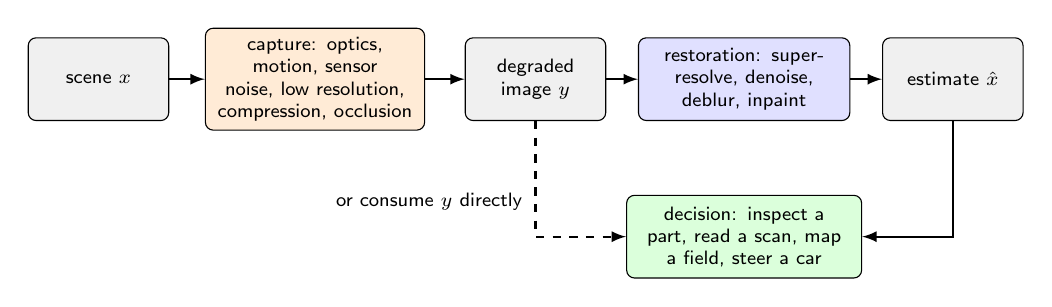
\begin{tikzpicture}[font=\sffamily\scriptsize, >=latex,
      box/.style={draw, rounded corners=0.1cm, align=center, minimum height=1.05cm},
      capbox/.style={box, fill=orange!16, text width=2.55cm},
      img/.style={box, fill=gray!12, text width=1.55cm},
      res/.style={box, fill=blue!12, text width=2.45cm},
      dec/.style={box, fill=green!14, text width=2.75cm}]
    \node[img] (scene) at (0,0) {scene $x$};
    \node[capbox] (capture) at (2.75,0) {capture: optics, motion, sensor noise, low resolution, compression, occlusion};
    \node[img] (y) at (5.55,0) {degraded\\image $y$};
    \node[res] (restore) at (8.2,0) {restoration: super-resolve, denoise, deblur, inpaint};
    \node[img] (xhat) at (10.85,0) {estimate $\hat{x}$};
    \node[dec] (decide) at (8.2,-2.0) {decision: inspect a part, read a scan, map a field, steer a car};
    \draw[->, thick] (scene) -- (capture);
    \draw[->, thick] (capture) -- (y);
    \draw[->, thick] (y) -- (restore);
    \draw[->, thick] (restore) -- (xhat);
    \draw[->, thick] (xhat.south) |- (decide.east);
    \draw[->, thick, dashed] (y.south) |- (decide.west);
    \node[font=\sffamily\scriptsize, align=center] at (4.2,-1.55) {or consume $y$ directly};
  \end{tikzpicture}\\[0.5em]
  {\scriptsize Restoration serves two readers: a person looking at the image, and a model making a decision from it.\par}
  \vspace{0.5em}
  \begin{itemize}\footnotesize\itemsep0.3em
    \item Restoration tries to invert the capture process. The decision stage inherits every error it leaves behind, including detail it invented.
    \item Today both stages start from large pretrained models: diffusion priors (covered earlier as generators) for restoration, and encoders such as DINOv2, CLIP and SAM (covered earlier), frozen or fine-tuned, for the decisions.
  \end{itemize}
\end{frame}

\begin{frame}{What Changed Since 2024}
  Where each part of today's lecture starts, and the 2024--2026 work it covers:\par
  \vspace{0.3em}
  {\centering\scriptsize
  \begin{tabular}{>{\raggedright\arraybackslash}p{2.1cm} >{\raggedright\arraybackslash}p{3.7cm} >{\raggedright\arraybackslash}p{6.6cm}}
    \toprule
    \textbf{Area} & \textbf{Reference point} & \textbf{2024--2026 developments covered today} \\
    \midrule
    Super-resolution & regression networks trained on synthetic pairs (SwinIR, HAT) & frozen diffusion priors steered by the input (DiffBIR, SUPIR), one-step models (OSEDiff), near-real-time streaming video (FlashVSR) \\
    \addlinespace[0.2em]
    Denoising, deblurring & one network per degradation & instruction-driven and agentic restorers; one generative prior for any known degradation (posterior sampling, refined in 2025) \\
    \addlinespace[0.2em]
    Inpainting & fill the hole from context (LaMa) & plug-in diffusion fill (BrushNet), removal of objects with their shadows and reflections (ObjectDrop, ROSE) \\
    \addlinespace[0.2em]
    Anomaly detection & one model per product (PatchCore) & one model per dataset (Dinomaly), zero- and few-shot CLIP and DINOv2 detectors, multimodal LLM inspectors \\
    \addlinespace[0.2em]
    Medical imaging & a U-Net configured per dataset (nnU-Net) & promptable 3D segmentation (MedSAM2, nnInteractive), pathology foundation models, an open medical VLM (MedGemma) \\
    \addlinespace[0.2em]
    Earth observation & supervised U-Nets per task; early pretraining (SatMAE) & multi-temporal and any-sensor foundation models (Prithvi-EO-2.0, DOFA, TerraMind), released embedding fields (AlphaEarth) \\
    \addlinespace[0.2em]
    Driving & modular stacks; UniAD joins them, scored open loop & diffusion and vision-language-action policies (DiffusionDrive, EMMA, Alpamayo-R1), non-reactive (NAVSIM) and closed-loop (Bench2Drive) scoring \\
    \bottomrule
  \end{tabular}\par}
\end{frame}

\begin{frame}{Constraints That Shape Deployed Vision}
  Five constraints recur in every setting of today's lecture:\par
  \vspace{0.5em}
  {\centering\scriptsize
  \begin{tabular}{>{\raggedright\arraybackslash}p{2.6cm} >{\raggedright\arraybackslash}p{4.6cm} >{\raggedright\arraybackslash}p{4.8cm}}
    \toprule
    \textbf{Constraint} & \textbf{Where it bites} & \textbf{Answer in this lecture} \\
    \midrule
    Few or no labels & defects are rare and unforeseen; one hand-drawn 3D lesion mask takes minutes & one-class anomaly detection; promptable and self-supervised medical models \\
    \addlinespace[0.25em]
    Distribution shift & a new scanner, a new satellite sensor, changed lighting, night & training on realistic degradations; sensor-agnostic Earth-observation models; closed-loop driving tests \\
    \addlinespace[0.25em]
    Compute budget & inspection at line rate, phones, roadside cameras & one-step diffusion restorers; millisecond anomaly detectors; open models that run locally \\
    \addlinespace[0.25em]
    Asymmetric error costs & a missed crack or tumour costs far more than a false alarm & thresholds set on validation data; pixel-level and region-level metrics \\
    \addlinespace[0.25em]
    Trust & generated detail can look right and be wrong & fidelity metrics next to perceptual ones; hallucination checks before use \\
    \bottomrule
  \end{tabular}\par}
  \vspace{0.6em}
  \begin{itemize}\footnotesize\itemsep0.3em
    \item Each section names representative recent model families and, where open weights exist, models an end user can run on a single consumer GPU or a CPU.
  \end{itemize}
\end{frame}
